\label{Chapter1}

\section{Χώροι χρώματος και κατάτμηση}

Σε αυτό το κεφάλαιο θα πραγματοποιηθεί ένα παράδειγμα ιστογράμματος και κατάτμησης για να μελετηθεί η διαφορά του RGB, του HSV και του συνδυασμού τους.

\subsection{Επιλογή εικόνας}

Η εικόνα η οποία επιλέχτηκε για να εκτελεστούν οι αλγόριθμοι πάνω της είναι η εικόνα του Σχήματος~\ref{fig:doctor}

\begin{figure}[H]
  \centering
  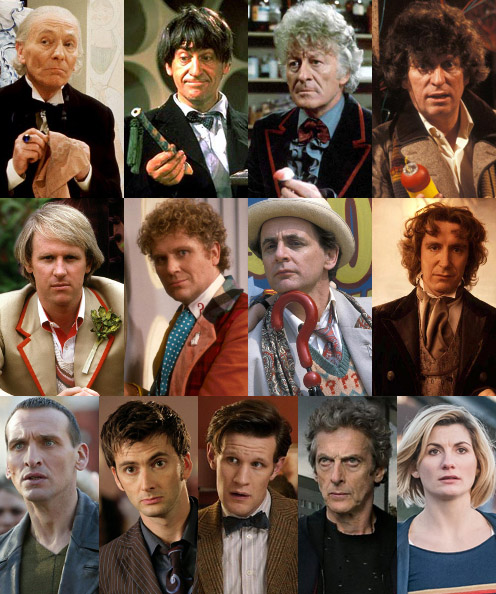
\includegraphics[width=100mm]{Figures/the_doctor}
  \caption[Τα 13 regenerations του Doctor]{Οι διάφορες μορφές (regenerations) του Doctor από την σειρά <<Doctor Who>> του BBC, 1963 - 1989 και 2005 - σήμερα}
  \label{fig:doctor}
\end{figure}

\subsubsection{3D plot της original RGB εικόνας}

Για να φορτωθεί η εικόνα στο script και να την θεωρήσει ως RGB χρειάζονται μερικές εντολές. Τα ακρώνυμα RGB σημαίνει Red (κόκκινο), Green (πράσινο) και Blue (Μπλε). Η OpenCV όμως τα διαβάζει ως BGR και θα πρέπει να γίνει η κατάλληλη μετατροπή σε RGB. Αυτό γίνετε με τον εξής τρόπο:

\begin{minted}{python}
image = cv2.imread('the_doctor.jpg')
image = cv2.cvtColor(image, cv2.COLOR_BGR2RGB)
\end{minted}

Για να πραγματοποιηθεί 3D plot, θα πρέπει να γίνει διαχωρισμός των καναλιών. Υπάρχει έτοιμη συνάρτηση στο OpenCV που το κάνει αυτόματα. Τα αποτελέσματα της συνάρτησης παρουσιάζονται στο Σχήμα~\ref{fig:rgb_3d_plot}.

\begin{figure}[H]
  \centering
  
\includegraphics[width=100mm]{Figures/rgb_3d}
  \caption{RGB 3D Plot}
  \label{fig:rgb_3d_plot}
\end{figure}

\subsubsection{Ιστόγραμμα της RGB εικόνας}

Το ιστόγραμμα είναι ένα πολύ δυνατό εργαλείο στην επεξεργασία εικόνας. Απεικονίζει την διαφορά των τιμών μίας εικόνας ανά κανάλι. Μπορεί να υπολογισθεί πολύ εύκολα χρησιμοποιώντας την βιβλιοθήκη NumPy.

\begin{minted}{py}
for channel_id, channel in zip(channel_ids, channels):
  histogram, bin_edges = np.histogram(image[:, :, channel_id], bins=bins, range=(0, bins))
\end{minted}

Τροποποιώντας λίγο τον κωδικά, μπορεί να εισαχθεί σε ένα plot. Το αποτέλεσμα του plot παρουσιάζεται στο Σχήμα~\ref{fig:rgb_histogram}.

\begin{minted}{py}
def plot_histogram(image, labels, bins,
                   title, filename, channels=('red', 'green', 'blue'),
                   channel_ids=(0, 1, 2)) -> None:
  plt.xlim([0, 256])

  for label, channel_id, channel in zip(labels, channel_ids, channels):
    histogram, bin_edges = np.histogram(
      image[:, :, channel_id],
      bins=bins,
      range=(0, bins)
    )
    plt.plot(bin_edges[0:-1], histogram, label=label, color=channel)

  plt.xlabel("Color value")
  plt.ylabel("Pixels")
  plt.title(title)
  plt.legend(loc="best")
  plt.savefig(f"{filename}.png")
  plt.show()

plot_histogram(image, ('Red', 'Green', 'Blue'), 256, "RGB Histogram", "rgb_histogram")
\end{minted}

\begin{figure}[H]
  \centering
  
\includegraphics[width=100mm]{Figures/rgb_histogram}
  \caption{RGB Histogram}
  \label{fig:rgb_histogram}
\end{figure}

\subsubsection{Κατάτμηση της RGB εικόνας}

Κατάτμηση είναι όταν μία εικόνα χωρίζεται σε μικρότερα τμήματα τα οποία είναι όμοια μαζί τους. Η κατάτμηση μπορεί να γίνει με πολλές μεθοδολογίες. Οι δύο που επιλέχτηκαν για το παράδειγμα είναι ο MeanShift και ο KMeans. Και οι δύο αλγόριθμοι είναι παρόμοιοι και κάνουν την ίδια δουλεία, εύρεση των clusters.

\begin{minted}{py}
def segment_image(image, color_code, channel_amount=3) -> None:
  shape = image.shape
  flat_image = np.reshape(image, [-1, channel_amount])

  # MeanShift segmentation
  bandwidth = estimate_bandwidth(flat_image, quantile=0.1, n_samples=100)
  meanshift = MeanShift(bandwidth=bandwidth, bin_seeding=True)
  meanshift.fit(flat_image)
  segmentation(flat_image, shape, color_code, channel_amount, meanshift, "MeanShift")

  # KMeans segmentation
  k_means = MiniBatchKMeans()
  k_means.fit(flat_image)
  segmentation(flat_image, shape, color_code, channel_amount, k_means, "KMeans")

segment_image(image, "RGB")
\end{minted}

\begin{figure}[H]
  \centering
  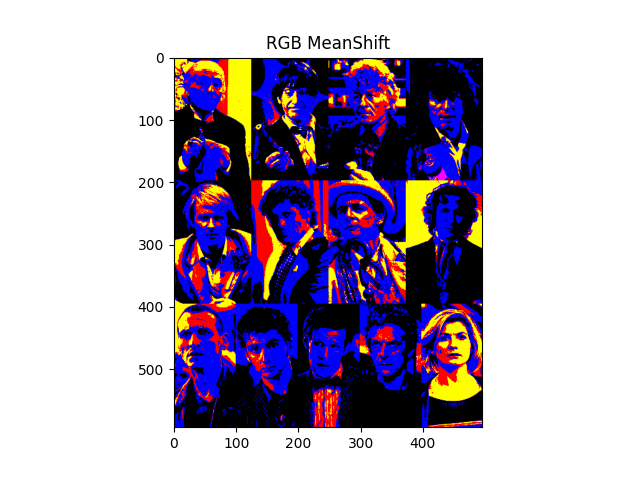
\includegraphics[width=100mm]{Figures/RGB_MeanShift}
  \caption{RGB MeanShift}
  \label{fig:rgb_meanshift}
\end{figure}

\begin{figure}[H]
  \centering
  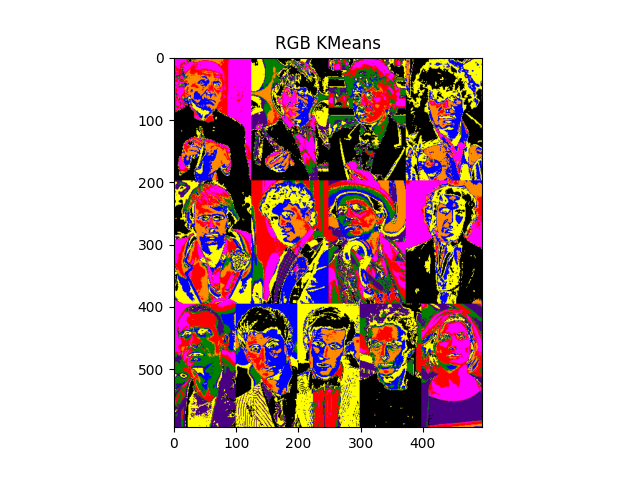
\includegraphics[width=100mm]{Figures/RGB_KMeans}
  \caption{RGB KMeans}
  \label{fig:rgb_kmeans}
\end{figure}

Στα Σχήματα~\ref{fig:rgb_meanshift} και ~\ref{fig:rgb_kmeans} απεικονίζονται τα αποτελέσματα των αλγορίθμων.

\subsection{Μετατροπή σε HSV και παρουσίαση αποτελεσμάτων}

Το HSV είναι ένας εναλλακτικός τρόπος αναπαράστασης της εικόνας. Τα ακρώνυμα είναι Hue (απόχρωση), Saturation (κορεσμός) και Value (τιμή). Η μετατροπή από RGB σε HSV είναι η εξής:

\begin{minted}{py}
hsv_image = cv2.cvtColor(image, cv2.COLOR_RGB2HSV)
save_image("hsv", hsv_image)
\end{minted}

Η εικόνα σε HSV παρουσιάζεται στο Σχήμα~\ref{fig:hsv}. Να παρατηρηθεί πόσο πολύ έχει τροποποιηθεί η εικόνα. Στα Σχήματα~\ref{fig:hsv_meanshift} και \ref{fig:hsv_kmeans} παρουσιάζονται τα αποτελέσματα των αλγορίθμων MeanShift και KMeans στην HSV εικόνα. Παρατηρείτε ότι τα αποτελέσματα έχουν επίσης τροποποιηθεί.

\begin{figure}[H]
  \centering
  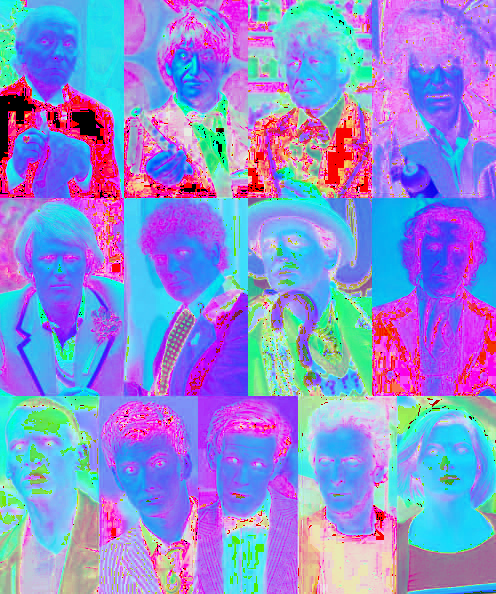
\includegraphics[width=100mm]{Figures/hsv}
  \caption{Η HSV εικόνα}
  \label{fig:hsv}
\end{figure}

\begin{figure}[H]
  \centering
  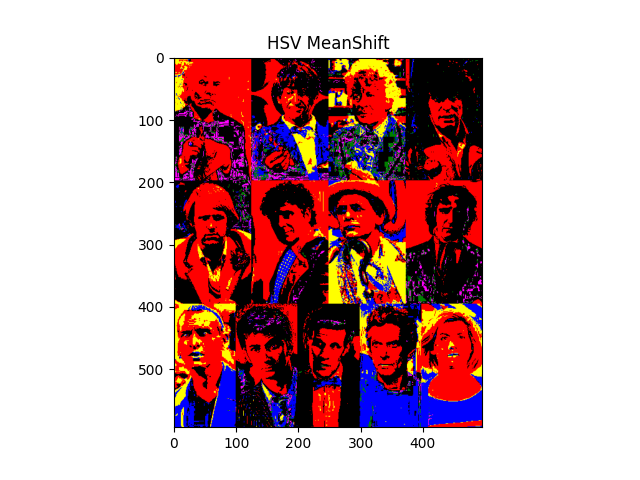
\includegraphics[width=100mm]{Figures/HSV_MeanShift}
  \caption{HSV MeanShift}
  \label{fig:hsv_meanshift}
\end{figure}

\begin{figure}[H]
  \centering
  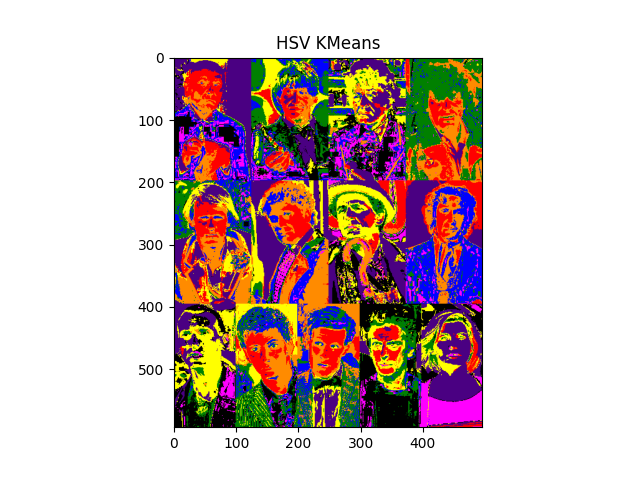
\includegraphics[width=100mm]{Figures/HSV_KMeans}
  \caption{HSV KMeans}
  \label{fig:hsv_kmeans}
\end{figure}

\subsection{Σχολιασμός αποτελεσμάτων RGB και HSV}
\label{paratiriseis}

Τα αποτελέσματα μεταξύ των δύο αλγορίθμων είτε ο KMeans είτε ο MeanShift είναι πολύ διαφορετικά μεταξύ τους με RGB και με το HSV. Ο MeanShift παράγει πολύ καλά με το RGB μοντέλο, ένω ο KMeans με το HSV μοντέλο.

\subsubsection{Συνδιασμός RGB και HSV}

Μπορεί να εξελιχθεί λίγο παραπάνω το ερώτημα συνδυάζοντας τα δύο μοντέλα και περνώντας τα από τους δύο αλγορίθμους. Ο αλγόριθμος που συνδυάζει τα δύο μοντέλα είναι ο εξής:

\begin{minted}{py}
combined_image = np.concatenate((image, hsv_image), axis=2)
\end{minted}

Στα Σχήματα~\ref{fig:rgb_hsv_meanshift} και ~\ref{fig:rgb_hsv_kmeans} φαίνονται τα αποτελέσματα των αλγορίθμων. Τα αποτελέσματα φαίνονται πολύ πιο καλύτερα από όταν ήταν ξεχωριστά τα μοντέλα.

\begin{figure}[H]
  \centering
  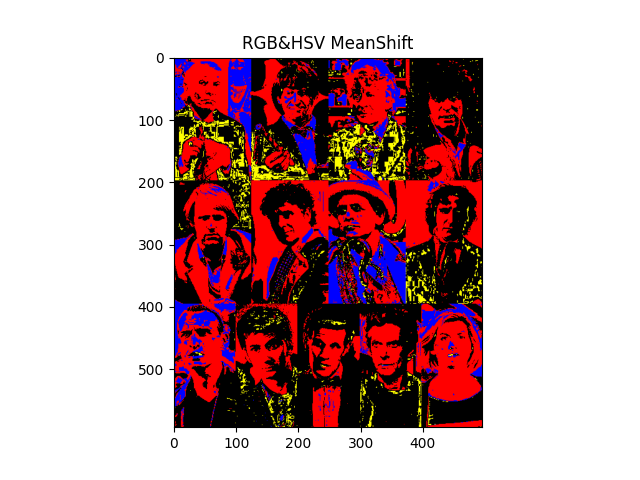
\includegraphics[width=100mm]{Figures/RGB&HSV_MeanShift}
  \caption{RGB και HSV MeanShift}
  \label{fig:rgb_hsv_meanshift}
\end{figure}

\begin{figure}[H]
  \centering
  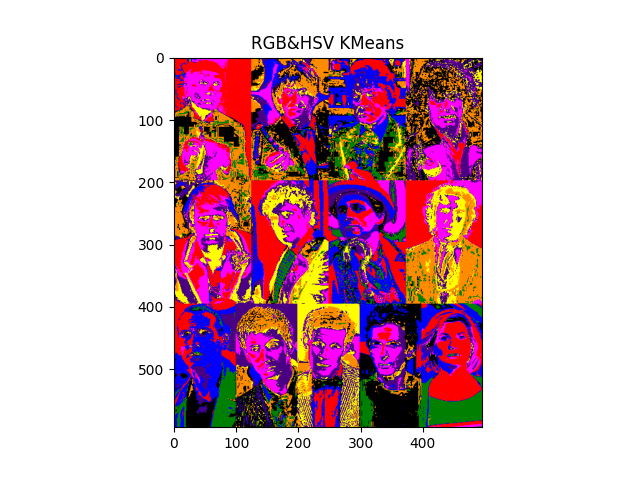
\includegraphics[width=100mm]{Figures/RGB&HSV_KMeans}
  \caption{RGB και HSV KMeans}
  \label{fig:rgb_hsv_kmeans}
\end{figure}

\subsection{Silhouette Coefficient}

Ο Silhouette Coefficient ή silhouette score είναι ένας αριθμός που καθορίζει το πόσο καλό είναι μία clustering τεχνική. Το εύρος τιμών του είναι από το $ -1 $ εώς το $ 1 $, όπου:

\begin{itemize}
  \item 1: τα clusters μεταξύ τους είναι αρκετά μακρυά και εύκολα αναγνωρίσιμα
  \item 0: τα clusters είναι τελείως διαφορετικά μεταξύ τους
  \item -1: τα clusters έχουν ρυθμιστεί λάθος
\end{itemize}

Μαθηματικά:

\begin{equation}
  SilhouetteScore = \frac{(b - a)}{max(a, b)}
\end{equation}

όπου:

\begin{itemize}
  \item το a είναι η μέση απόσταση των inter-cluster από κάθε σημείο
  \item το b είναι η μέση απόσταση όλων των clusters
\end{itemize}

\begin{table}[H]
  \centering
	\begin{tabular}{ | p{4cm} | p{4cm} | p{6cm} | }
		\hline
		\textbf{Όνομα εικόνας} & \textbf{Αριθμός clusters} & \textbf{Αποτέλεσμα Silhouette} \\
		\hline
		RGB MeanShift & 5 & 0.43829281680682963 \\
		\hline
		RGB KMeans & 8 & 0.39261542176396413 \\
		\hline
		HSV MeanShift & 6 & 0.27099304439301336 \\
		\hline
    HSV KMeans & 8 & 0.3545841420133397 \\
    \hline
    RGB και HSV MeanShift & 4 & 0.262483435384828 \\
    \hline
    RGB και HSV KMeans & 8 & 0.33426919705784475 \\
    \hline
	\end{tabular}
  \caption[Αποτελέσματα Silhouette]{Tα αποτελέσματα που γύρισε ο αλγόριθμος φαίνονται στον παρακάτω πίνακα. Οι παρατηρήσεις που έγιναν στο Κεφάλαιο~\ref{paratiriseis} φαίνονται να επιβεβαιώνονται με τα αποτελέσματα.}
  \label{tab:silhouette}
\end{table}
